% !TeX root = ../thuthesis-example.tex

\chapter{实验结果与分析}

\section{数据集介绍}

本文主要在仿真数据上进行了实验,后续则将会在实验室采集的真实数据集 OpenIllumination\cite{liu2024openillumination} 上进行实验。由于数据对于逆渲染而言非常关键,我们需要在适合的数据集上进行测试。例如,我们的材质模型较为简化,因而无法处理透明物体。此外,我们希望环境光尽量接近自然光,过强和过弱的光源都会给逆渲染带来巨大挑战。前者会导致过分曝光,从而无法判断物体表面的真实颜色,后者则会导致过量阴影。

基于上述原因,我们选择了三维重建领域常见仿真数据集 Nerf-synthetic\cite{nerf} 数据集,并按照我们的需求,将三维场景进行了重新渲染。我们采用了统一的环境光映射,如图 \ref{fig:envmap} 所示。

\begin{figure}
  \centering
  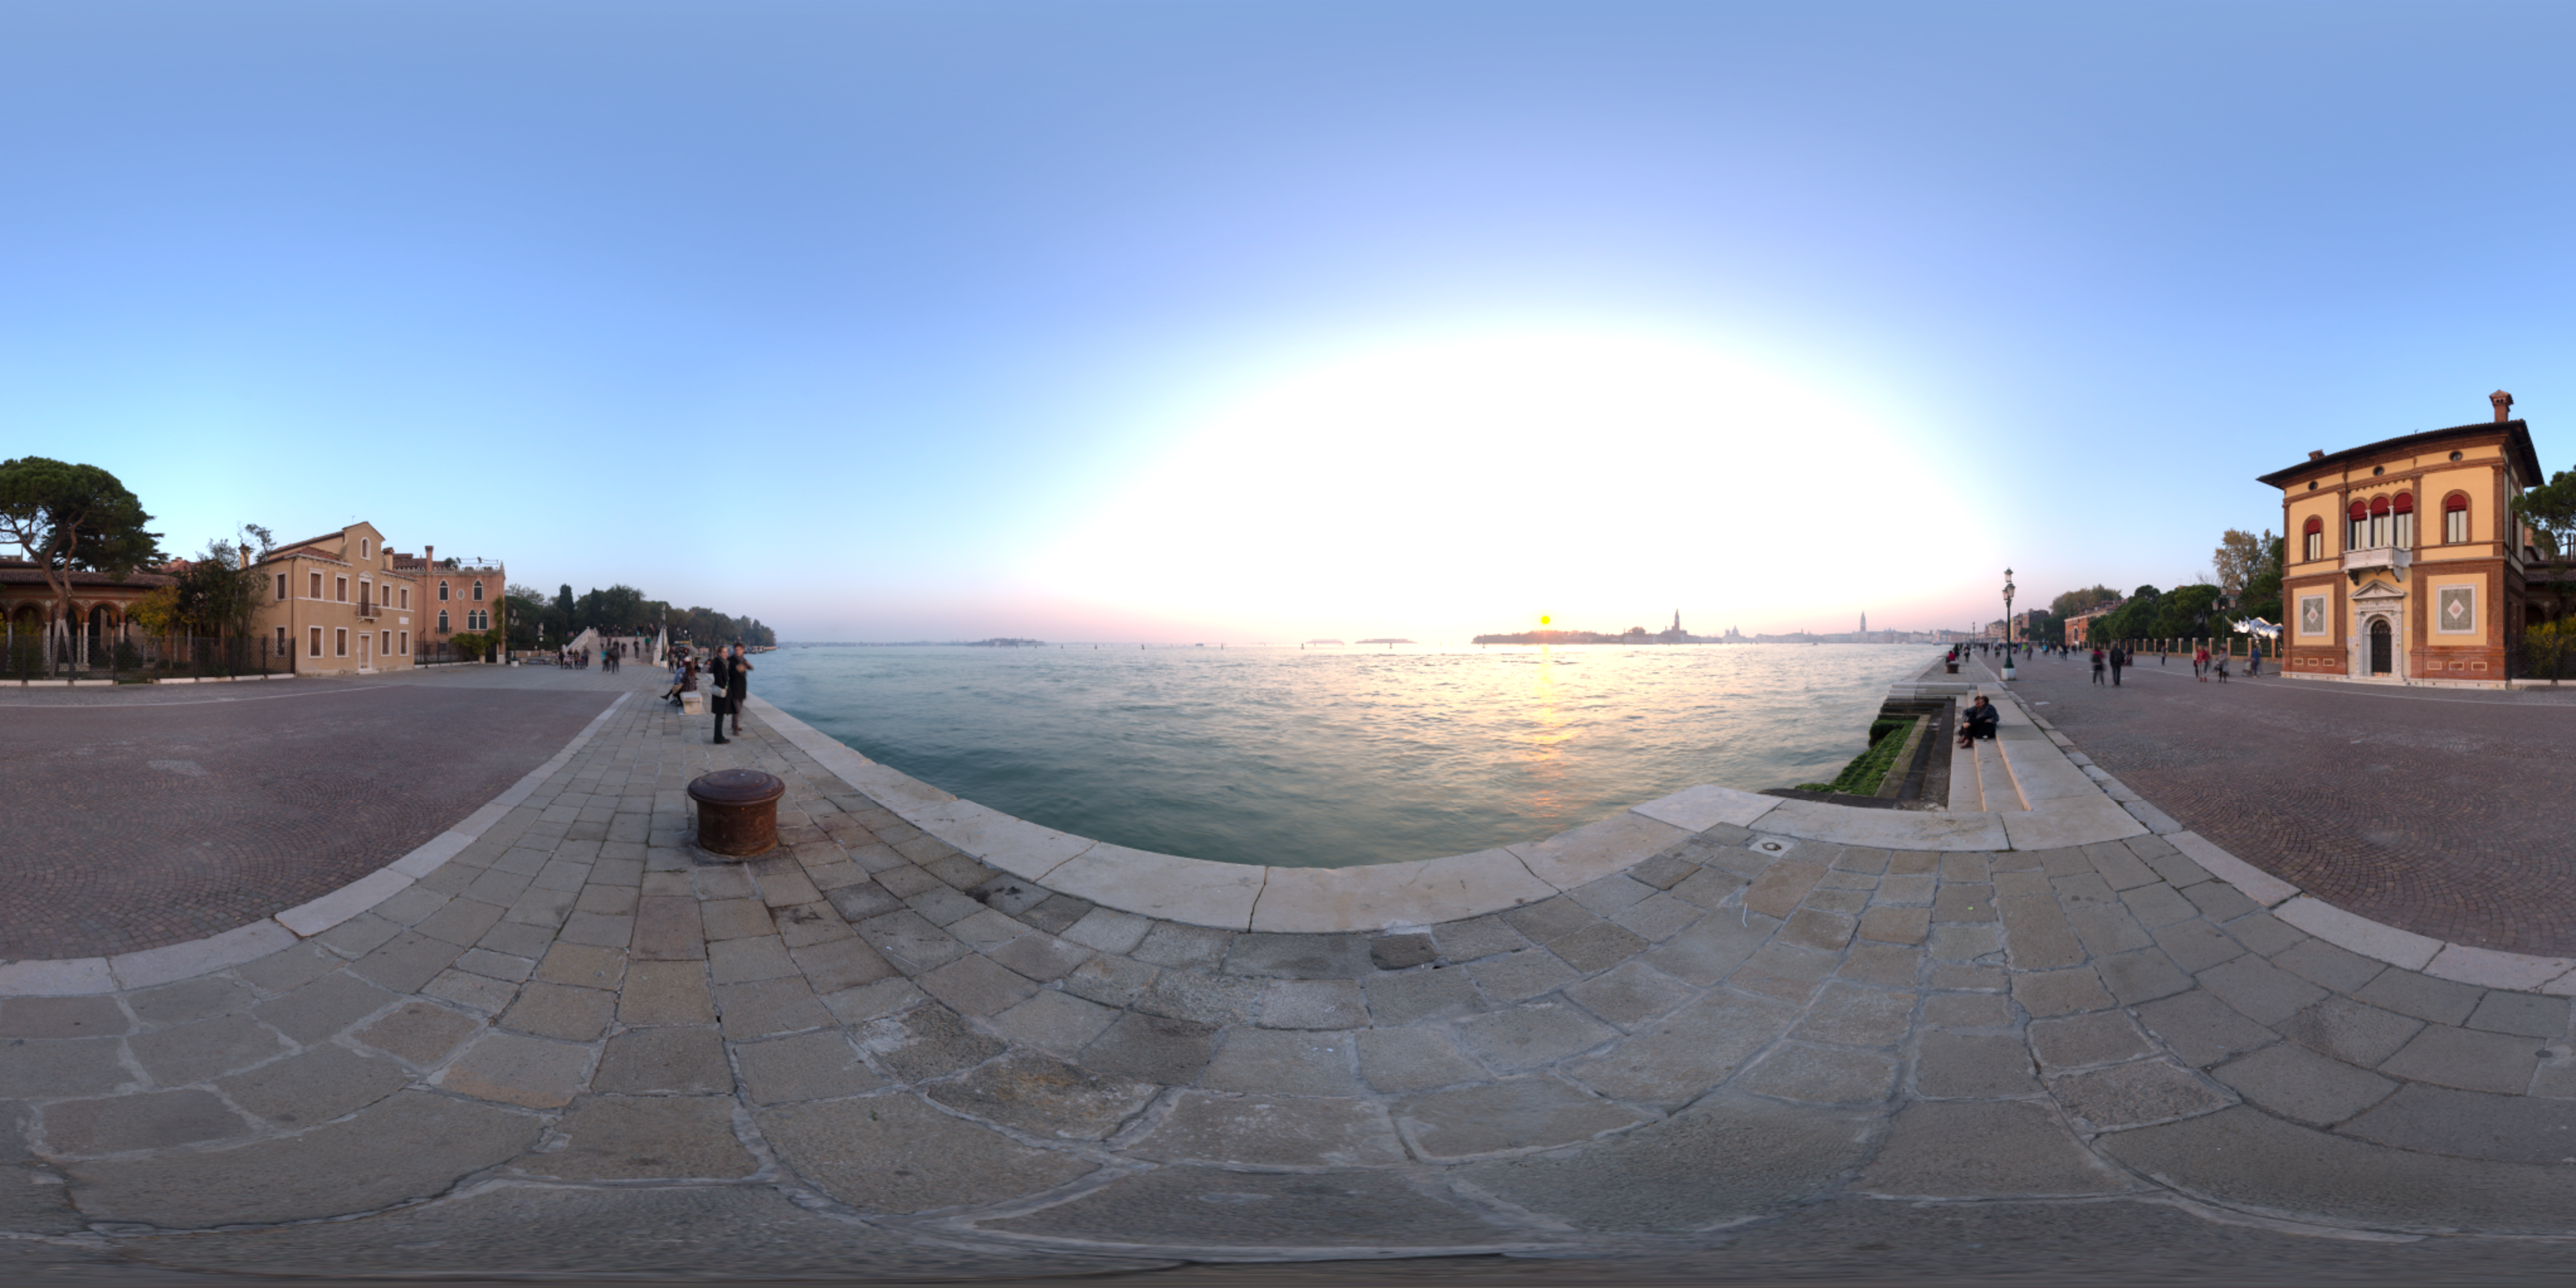
\includegraphics[width=0.8\linewidth]{envmap.pdf}
  \caption{环境光图}
  \label{fig:envmap}
\end{figure}

理论上说,我们期望用我们自己实现的光线追踪器完成数据的渲染过程。这是因为渲染并没有理论上的正确与错误之分,生成数据与训练使用相同的渲染器可以保证渲染过程的一致性,从而尽可能还原真实材质。然而,由于我们的光线追踪器的实现尚未完全,我们暂时使用了 Blender \cite{blender} 进行重新渲染。

Nerf-synthetic 包含八个场景,分别是热狗、材质、植物、乐高、麦克风、鼓、椅子和船。每个场景对应了 400 组相机参数,也即400 个不同视角,按照数据集原始设置,分为训练集、验证集和测试集三个部分,分别包含 100、100 和200组相机参数。渲染图片分辨率为 $800\times 800$。

由于时间限制并考虑到模型本身涉及到的材料、三维几何复杂度等,我们选择了其中的三个模型进行实验,分别是热狗、乐高和植物。这三个模型的复杂度适中,且包含了不同的材质,可以很好地验证我们的模型的有效性。

\begin{figure}
  \centering
  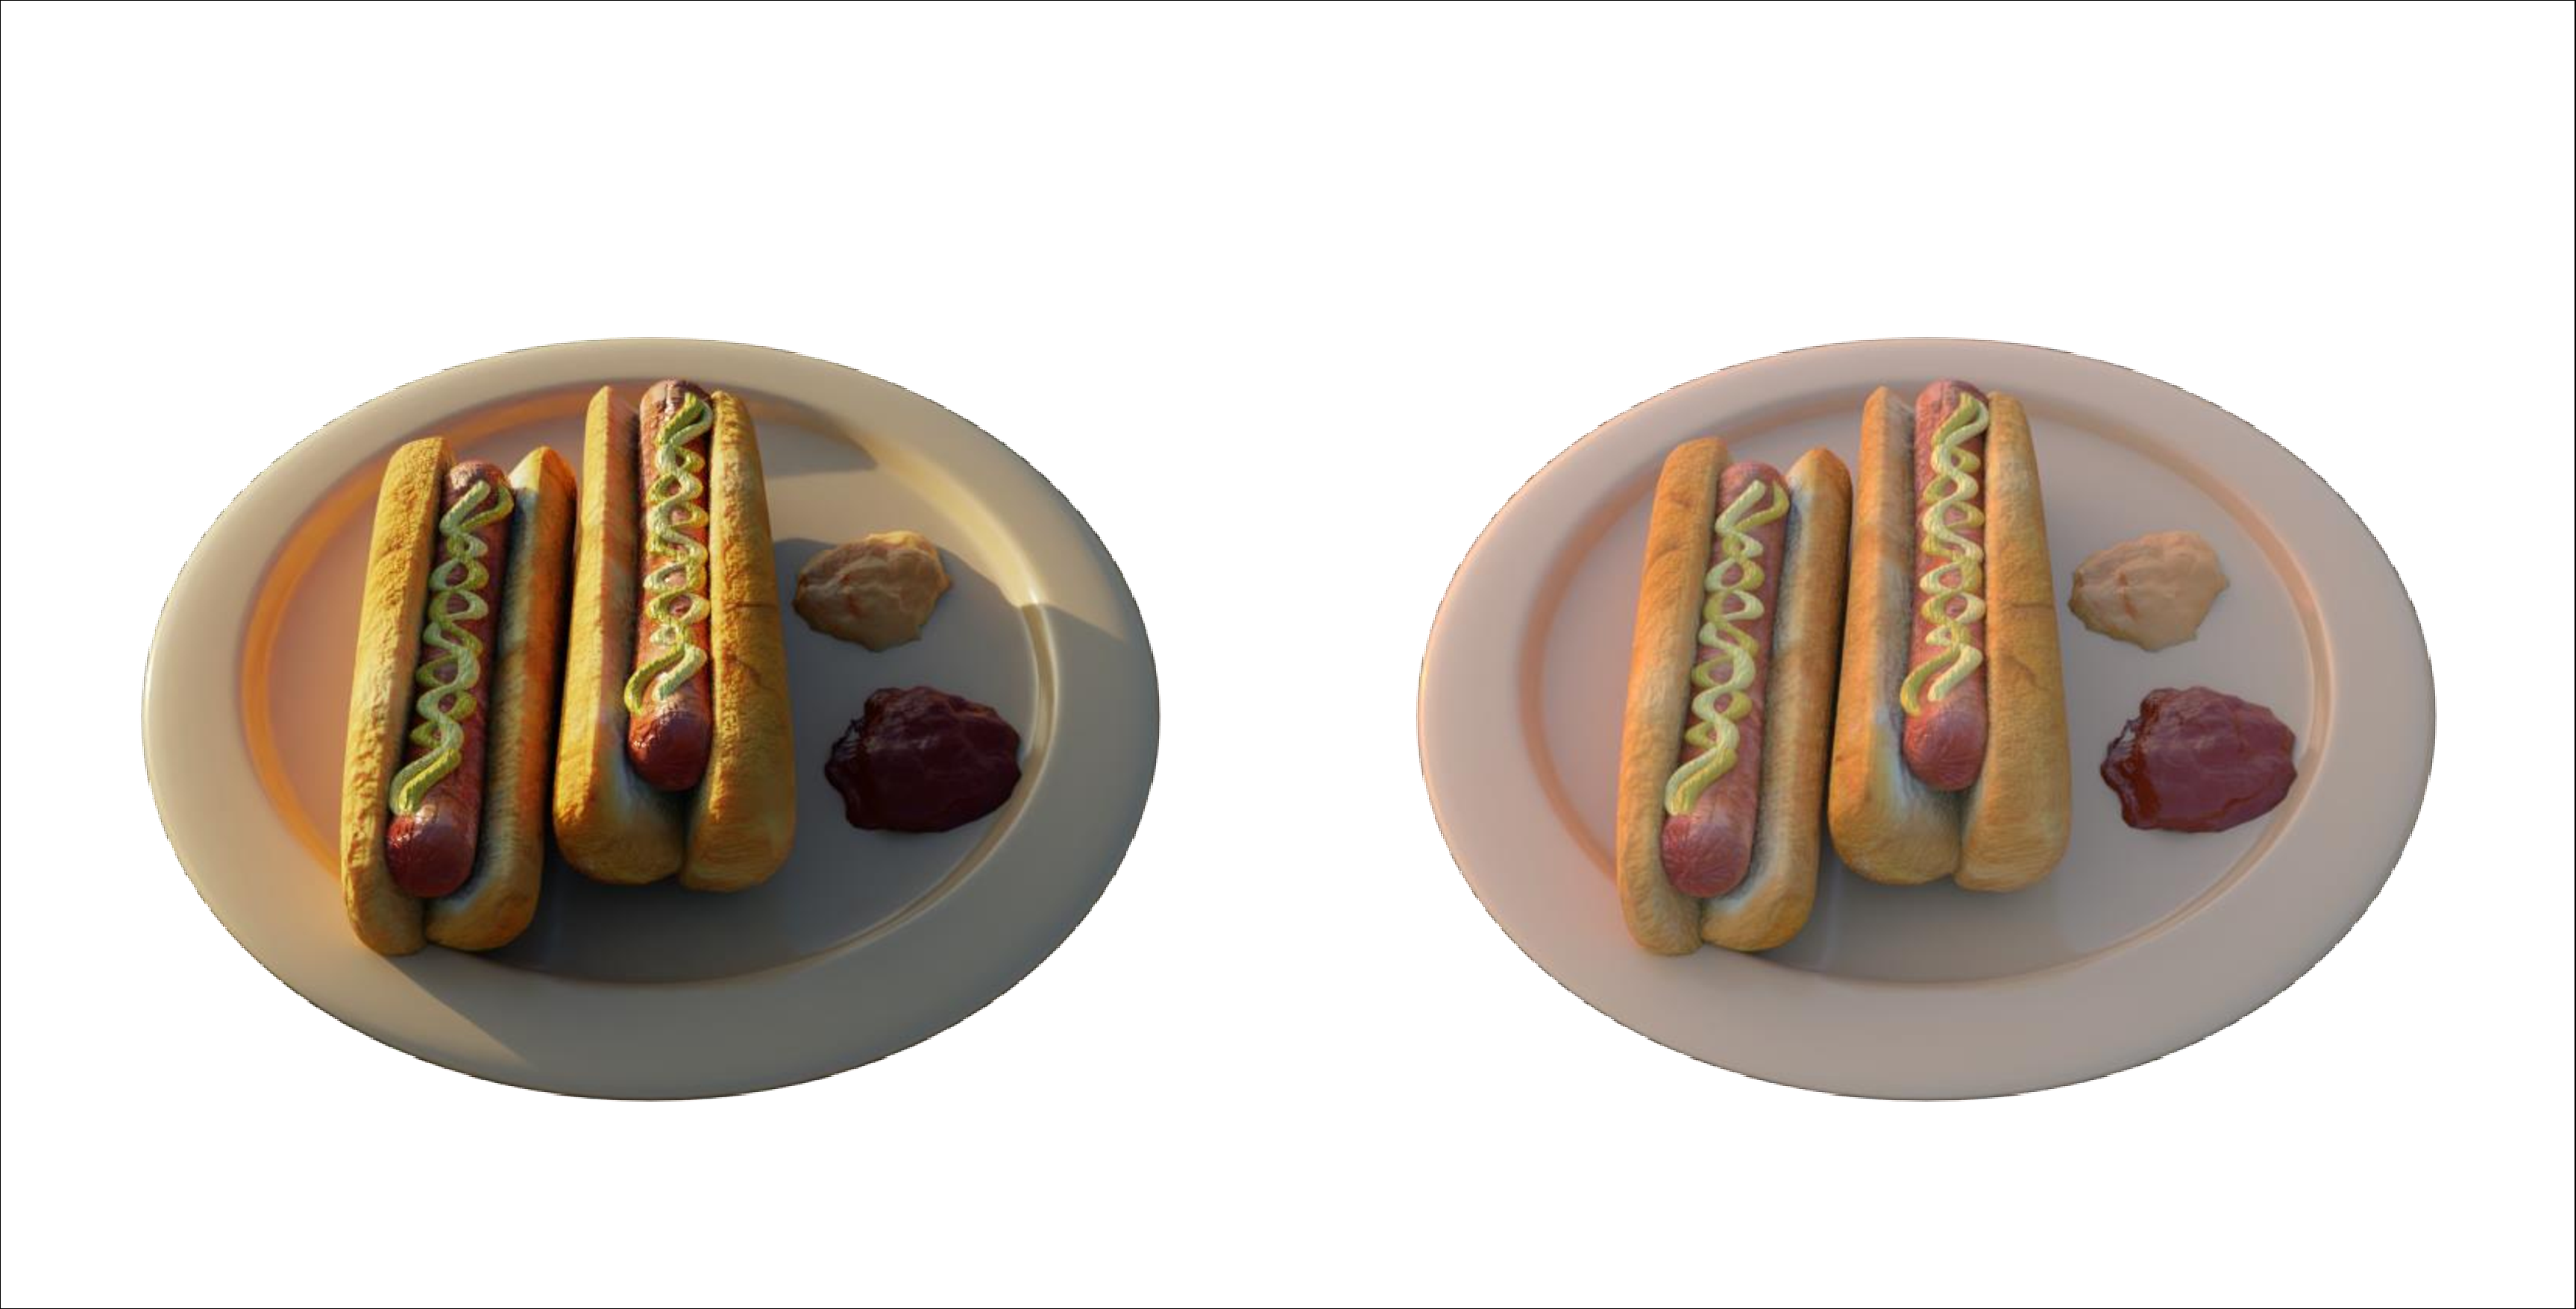
\includegraphics[width=0.8\linewidth]{cmp.pdf}
  \caption{原始数据和我们重新渲染的数据对比}
  \label{fig:cmp}
\end{figure}

图 \ref{fig:cmp} 中展示了原始的 Nerf-synthetic 的原始数据和我们重新渲染结果对比。可以看到,左侧原始数据中有大片的阴影,这对逆渲染并不友好。右侧重新渲染的数据在保留部分阴影的同时,光照更加均匀。

\section{评价指标}

针对我们的任务,我们需要衡量如下几个指标:

\begin{itemize}
  \item 新视角合成的图像质量。新视角合成是三维重建和逆渲染中最常见的任务之一。我们需要根据给定的新的相机参数,合成对应视角下的图像,并与该视角下的真实图像比较。我们通常使用 SSIM 和 PSNR 作为评价指标。
  \item 材质的准确度。我们的模型旨在恢复真实材质信息。因此,我们还将设计新的指标用于评估重建的材质信息与真实材质信息之间的相似度。
\end{itemize}

\subsection{峰值信噪比(Peak Signal-to-Noise Ratio,PSNR)}

PSNR 是通过直接比较原始图像和重建图像之间的像素值差异来衡量图像质量的。PSNR的计算基于均方误差(MSE),即重建图像与原始图像之间像素值的平方差的平均值。PSNR值通常以分贝(dB)为单位表示,值越高表示图像质量越好。

给定一个大小为 $m \times n$ 的图像 $I$,设真实图像为 $I_0$,均方差(MSE)定义为:
\begin{equation}
  \text{MSE}(I, I_0) = \frac{1}{mn} \sum_{i=1}^m \sum_{j=1}^n (I(i, j) - I_0(i, j))^2,
\end{equation}
峰值信噪比(PSNR)定义为:
\begin{equation}
  \text{PSNR}(I, I_0) = 10 \log_{10} \left( \frac{\max^2_I}{\text{MSE}(I, I_0)} \right).
\end{equation}

其中,$\max_I$ 表示图像 $I$ 中像素值范围的最大值。例如如果用 $[0,1]$ 中的实数表示像素值,那么 $\max_I = 1$。如果用 $[0,255]$ 中的整数表示像素值,那么 $\max_I = 255$。

\subsection{结构相似性指标(Structural Similarity Index,SSIM)}

SSIM 是一种结构相似性指标,它考虑了亮度、对比度和结构之间的相似性。SSIM 的取值范围是 $[0,1]$,其中 $1$ 表示完全相似,$0$ 表示完全不同。SSIM 指标的优点之一是它对人类视觉系统的影响较好地进行了建模,因此在许多情况下能够更好地预测人类主观感知的图像质量。SSIM 的计算公式如下:
\begin{equation}
  \text{SSIM}(I, I_0) = \frac{(2\mu_I\mu_{I_0} + C_1)(2\sigma_{I,I_0} + C_2)}{(\mu_I^2 + \mu_{I_0}^2 + C_1)(\sigma_I^2 + \sigma_{I_0}^2 + C_2)},
\end{equation}
其中,$\mu_I$ 和 $\mu_{I_0}$ 分别是图像 $I$ 和 $I_0$ 的均值,$\sigma_I^2$ 和 $\sigma_{I_0}^2$ 分别是图像 $I$ 和 $I_0$ 的方差,$\sigma_{I,I_0}$ 是图像 $I$ 和 $I_0$ 的协方差,$C_1$ 和 $C_2$ 是常数,用于避免分母为零。

\subsection{材质相似性指标}

观察图 \ref{fig:bakedshadow} 可以看到,我们得到的材质和真实材质的颜色似乎大相径庭。这是因为逆渲染本身的不适定性,最终渲染结果的颜色是由材质和光照相互作用决定的,并且有多组材质和光照参数可以得到相同的渲染结果。例如,假定光照为纯红色光,那么材质的颜色的绿色分量对于最终渲染结果就是无关紧要的。因此,直接比较我们还原的材质和真实材质图是不合理的。

我们首先根据真实材质图对我们得到的漫反射颜色进行修正。我们计算两者的平均颜色,然后将我们得到的漫反射颜色乘以两者的比值。在统一二者均值后,我们计算两者的 PSNR 作为材质相似性指标。

\newpage
\section{实验设置}

我们重新渲染的图片分辨率依然为 $800 \times 800$。

第一阶段我们使用了自己实现的修改版 TensoIR,其性能与官方的实现对比见表\ref{tab:tensoir}。可以看到,平均性能有微小的提升。此外,在三个场景中,仅仅最为容易的热狗场景上,指标稍有下降,而在其余两个较难的场景中性能都有所提升。我们的实现方差更小,更加稳定。
\begin{table}[h]
  \centering
  \begin{tabular}{ccccc}
  \toprule
  \textbf{测试集基于物理的渲染的 psnr} & 乐高  & 热狗 & 植物 & 平均 \\
  \midrule
  \textbf{原版 TensoIR}   & 34.7  & 36.82  & 29.78 & 33.77 \\
  \textbf{修改版 TensoIR} & 35.24 & 36.26  & 29.94 & 33.81 \\
  \bottomrule
  \end{tabular}
  \caption{官方实现的 TensoIR 和修改版 TensoIR 结果对比}
  \label{tab:tensoir}
\end{table}

对于第二阶段训练,由于显存限制,我们对输入图像做了裁剪处理。原始图像的大小是 $800 \times 800$ 像素,我们将其分成 $4 \times 4 = 16$ 块,每块大小为 $200 \times 200$ 像素。第三阶段训练中,同样由于显存限制,我们将图像分为 $2\times 2=4$ 块,每块分辨率 $400 \times 400$,并使用 $\text{spp}=128$ 以及 $\mathrm{depth}=6$。第二阶段和第三阶段训练都采用 $10000$ 次迭代。在第二阶段训练中,我们使用了 $256$ 分辨率的 DiffMC。

所有实验都在一块 NVIDIA RTX 4090 GPU 上进行。

\section {新视角合成结果及比较}

在表\ref{tab:psnr} 和 \ref{tab:ssim} 中,我们展示了新视角合成任务上我们的模型与现有一些其他逆渲染模型的结果比较。其中 TensoIR(DT)指直接将密度场按照 3.3.2.1 节中的可微 Marching Cube 转化为三维网格表示形式并渲染得到的结果。

可以看到,我们的模型在阶段二结束后,相比于现有其他方法,平均 PSNR有所提升。我们的模型可以得到高质量水密流形三维网格表示的同时,能够获得精细的纹理和环境光照信息,在新视角重建任务上表现优异。

注意到,在并入第三阶段后,模型在新视角合成任务上的能力有所下降。这是因为第三阶段的目标是消除烘焙到纹理中的照明伪影。照明伪影的存在原因是,通过这些看似“错误”的材质信息,我们可以得到更好的渲染质量。这些照明伪影通过更改物体表面颜色模拟遮挡与阴影,从而使得渲染结果更加真实。然而,真实的材质信息是更为关键的。例如在重渲染时更改环境光照,或是在几何编辑时更改物体几何信息,所有的遮挡和阴影都会改变。此时,再使用这些带有照明伪影的材质信息,会导致渲染结果与真实图像产生巨大差距。因此,在引入第三阶段后,通过牺牲少量渲染质量带来模型材质还原的提升是合理且有效的。

\begin{table}[h]
  \centering
  \begin{tabular}{ccccc}
    \toprule
                                   & 乐高                        & 热狗                        & 植物                        & 平均                        \\
                                   \midrule
  \multicolumn{1}{l}{TensoIR (DT)} & \multicolumn{1}{l}{26.78} & \multicolumn{1}{l}{28.90} & \multicolumn{1}{l}{21.86} & \multicolumn{1}{l}{25.85} \\
  PhySG                            & 19.81                     & 22.57                     & 18.40                     & 20.26                     \\
  Nvdiffrec                        & 30.14                     & 34.04                     & \textbf{29.88}                     & 31.02                     \\
  \midrule
  阶段一+二                            & \textbf{32.35}                     & \textbf{34.32}                     & 29.31                     & \textbf{31.99}                     \\
  阶段一+二+三                          & 31.40                     & 32.98                     & 27.12                     & 30.50              \\
  \bottomrule
  \end{tabular}
  \caption{新视角合成任务上的 PSNR 比较}
  \label{tab:psnr}
\end{table}

\begin{table}[h]
  \centering
  \begin{tabular}{ccccc}
    \toprule
                                   & 乐高                        & 热狗                        & 植物                        & 平均                        \\
                                   \midrule
  \multicolumn{1}{l}{TensoIR (DT)} & \multicolumn{1}{l}{0.897} & \multicolumn{1}{l}{0.914} & \multicolumn{1}{l}{0.913} & \multicolumn{1}{l}{0.908} \\
  PhySG                            & 0.771                     & 0.909                     & 0.838                     & 0.839                     \\
  Nvdiffrec                        & 0.941                     & 0.971                     & 0.968                     & 0.957                     \\
  \midrule
  阶段一+二                            & \textbf{0.977}                     & \textbf{0.979}                     & \textbf{0.978}                     & \textbf{0.978}                     \\
  阶段一+二+三                          & 0.949                     & 0.952                     & 0.904                     & 0.935            \\

  \bottomrule
  \end{tabular}
  \caption{新视角合成任务上的 SSIM 比较}
  \label{tab:ssim}
\end{table}

\section{材质相似性指标结果及比较}

在表\ref{tab:mat} 中,我们展示了材质相似性指标的实验结果和比较。这个实验主要是为了检验去除照明伪影的效果,因此我们在引入第三阶段训练前后进行了实验。

\begin{table}[h]
  \centering
  \begin{tabular}{ccccc}
    \toprule
          & 乐高    & 热狗    & 植物    & 平均    \\
          \midrule
  阶段一+二   & 21.18 & 23.83 & \textbf{21.37} & 22.13 \\
  阶段一+二+三 & \textbf{21.95} & \textbf{24.10} & 21.32 & \textbf{22.46} \\
  \bottomrule
  \end{tabular}
  \caption{材质相似性指标实验结果}
  \label{tab:mat}
\end{table}

\newpage
可以看到,引入第三阶段训练后,材质相似性指标有所提升。我们可以通过图\ref{fig:albedo} 更为明显的看到这一点。图中的三列从左至右分别代表 \textbf{不加入第三阶段训练的漫反射颜色图像}、\textbf{真实漫反射图像}和 \textbf{加入第三阶段训练的漫反射颜色图像}。第一排是模型训练得到的结果,第二排则是根据真实漫反射颜色图像进行颜色修正后的结果。可以看到,第一张图像中两条热狗之间以及盘子下方明显的阴影均已被减弱乃至消除。
\begin{figure}
  \centering
  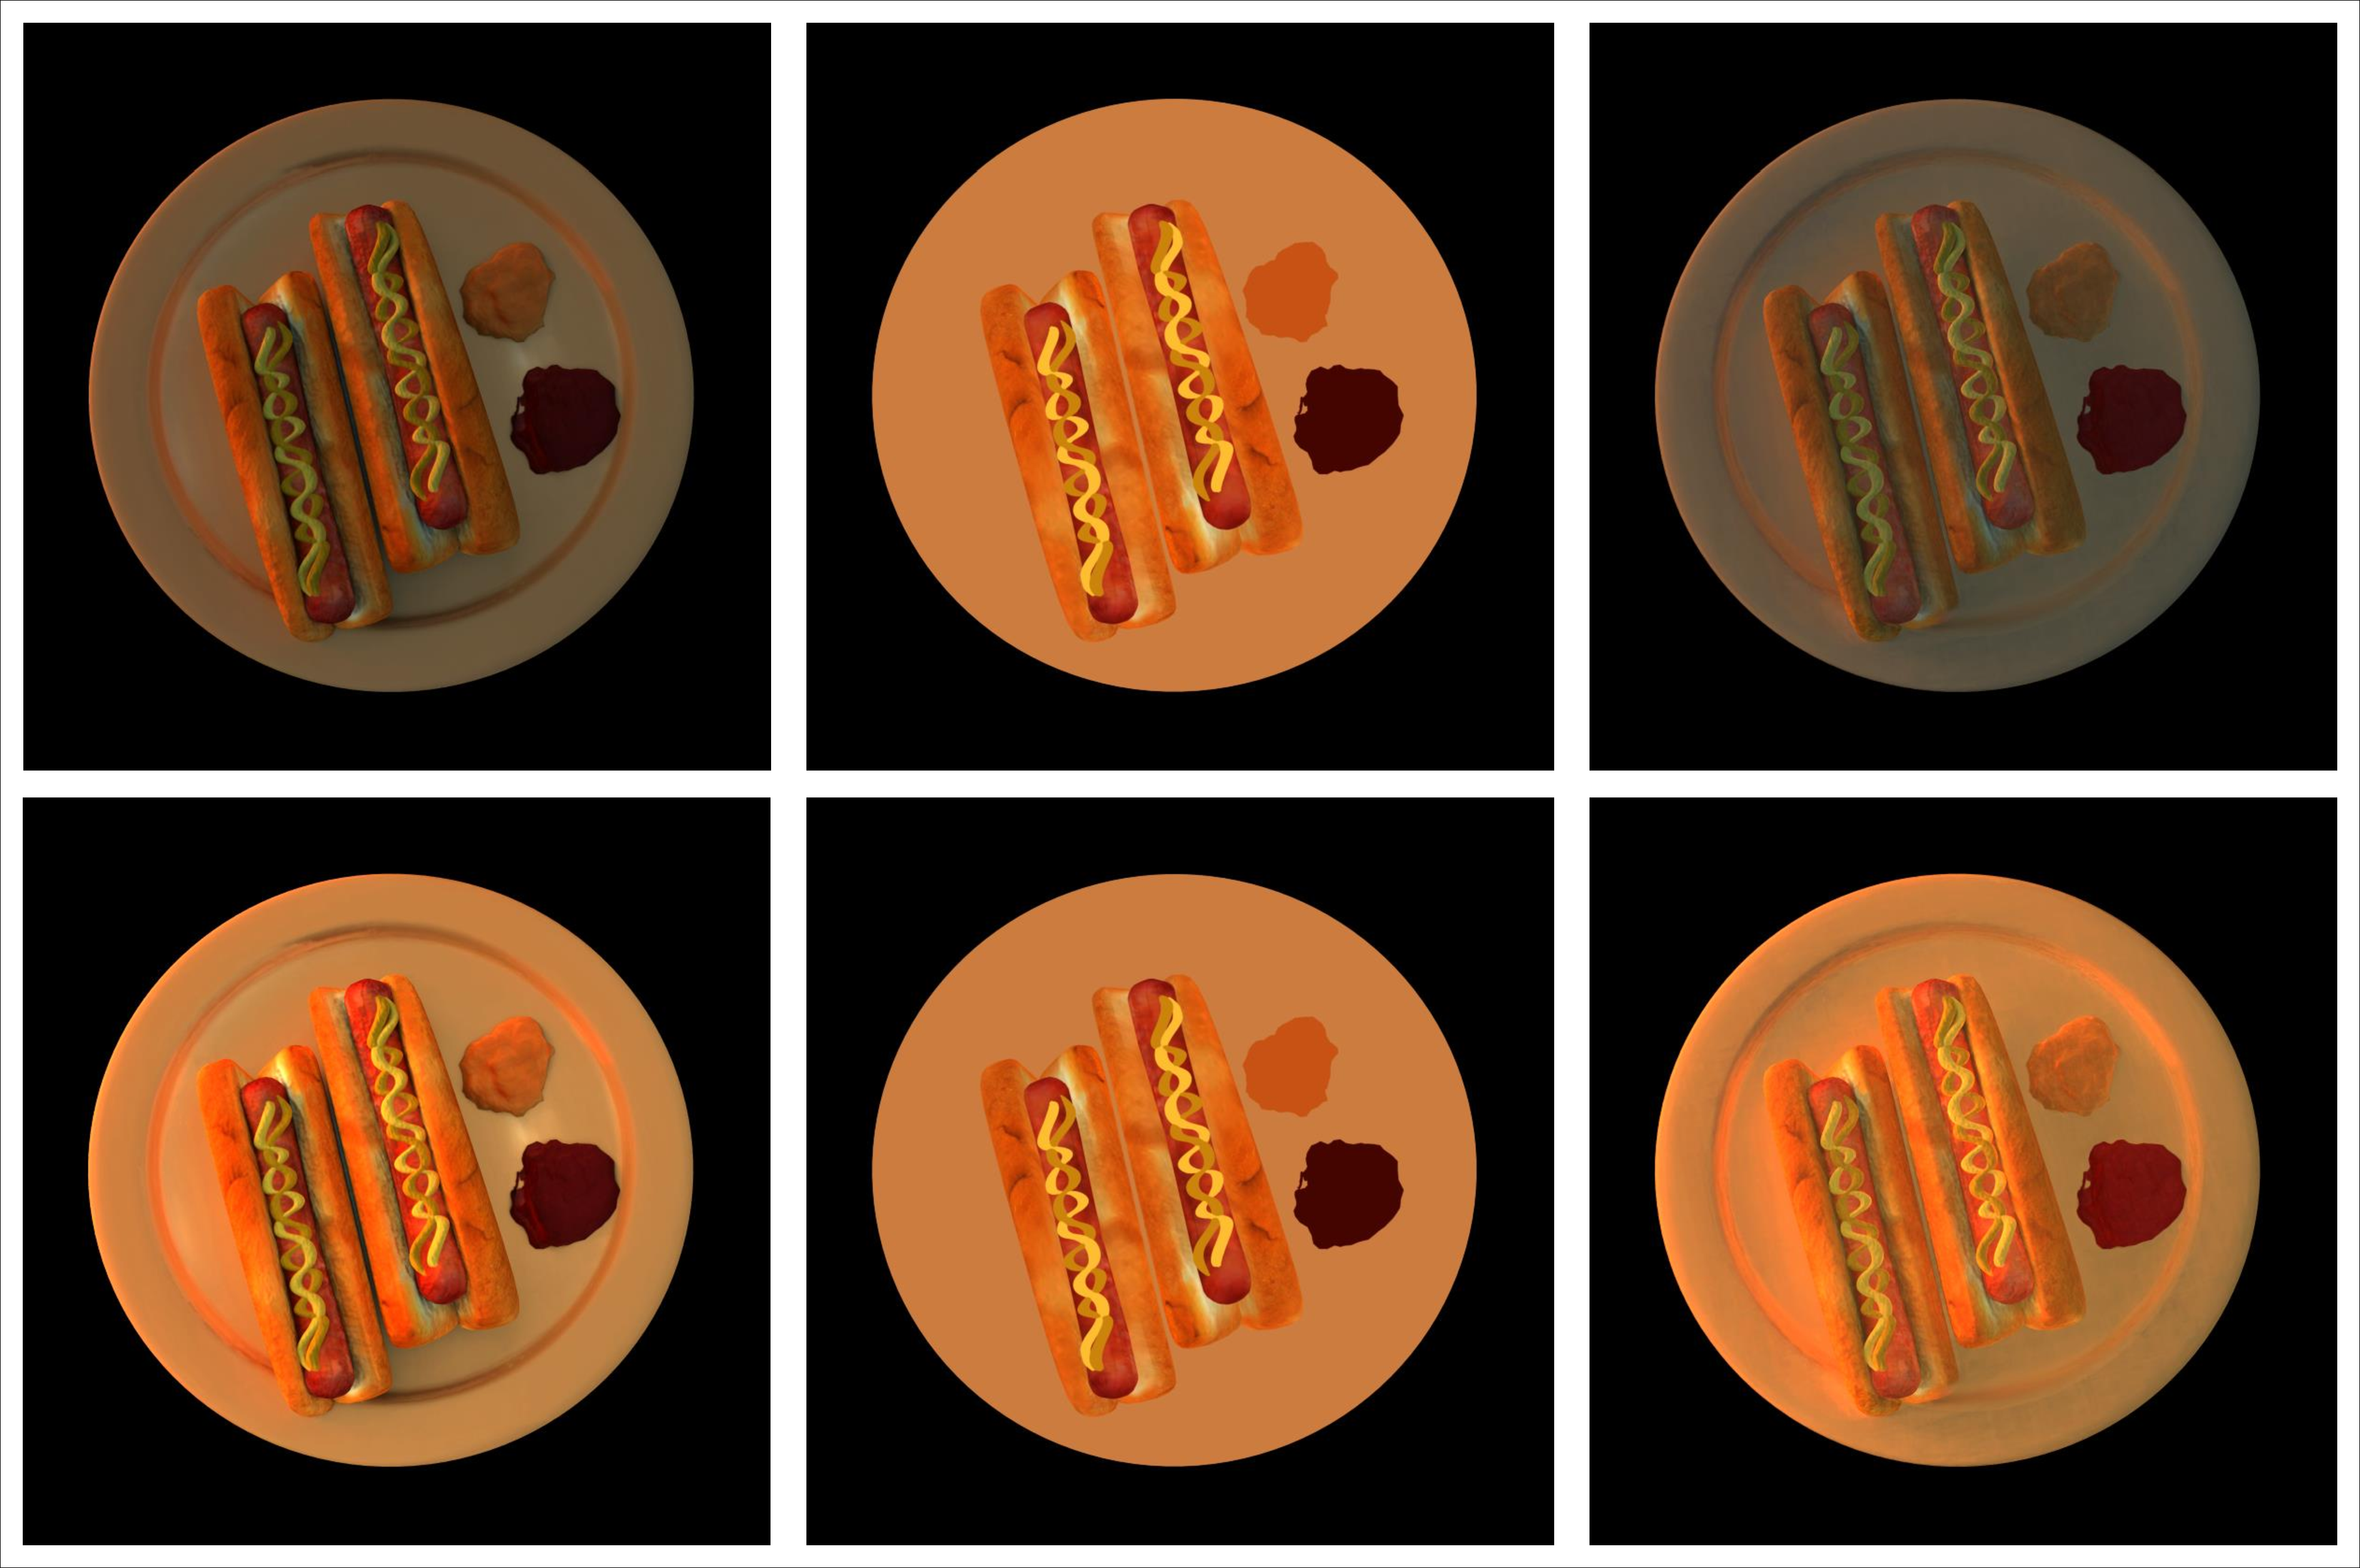
\includegraphics[width=\linewidth]{albedo.pdf}
  \caption{漫反射颜色比较}
  \label{fig:albedo}
\end{figure}

\begin{figure}[h]
  \centering
  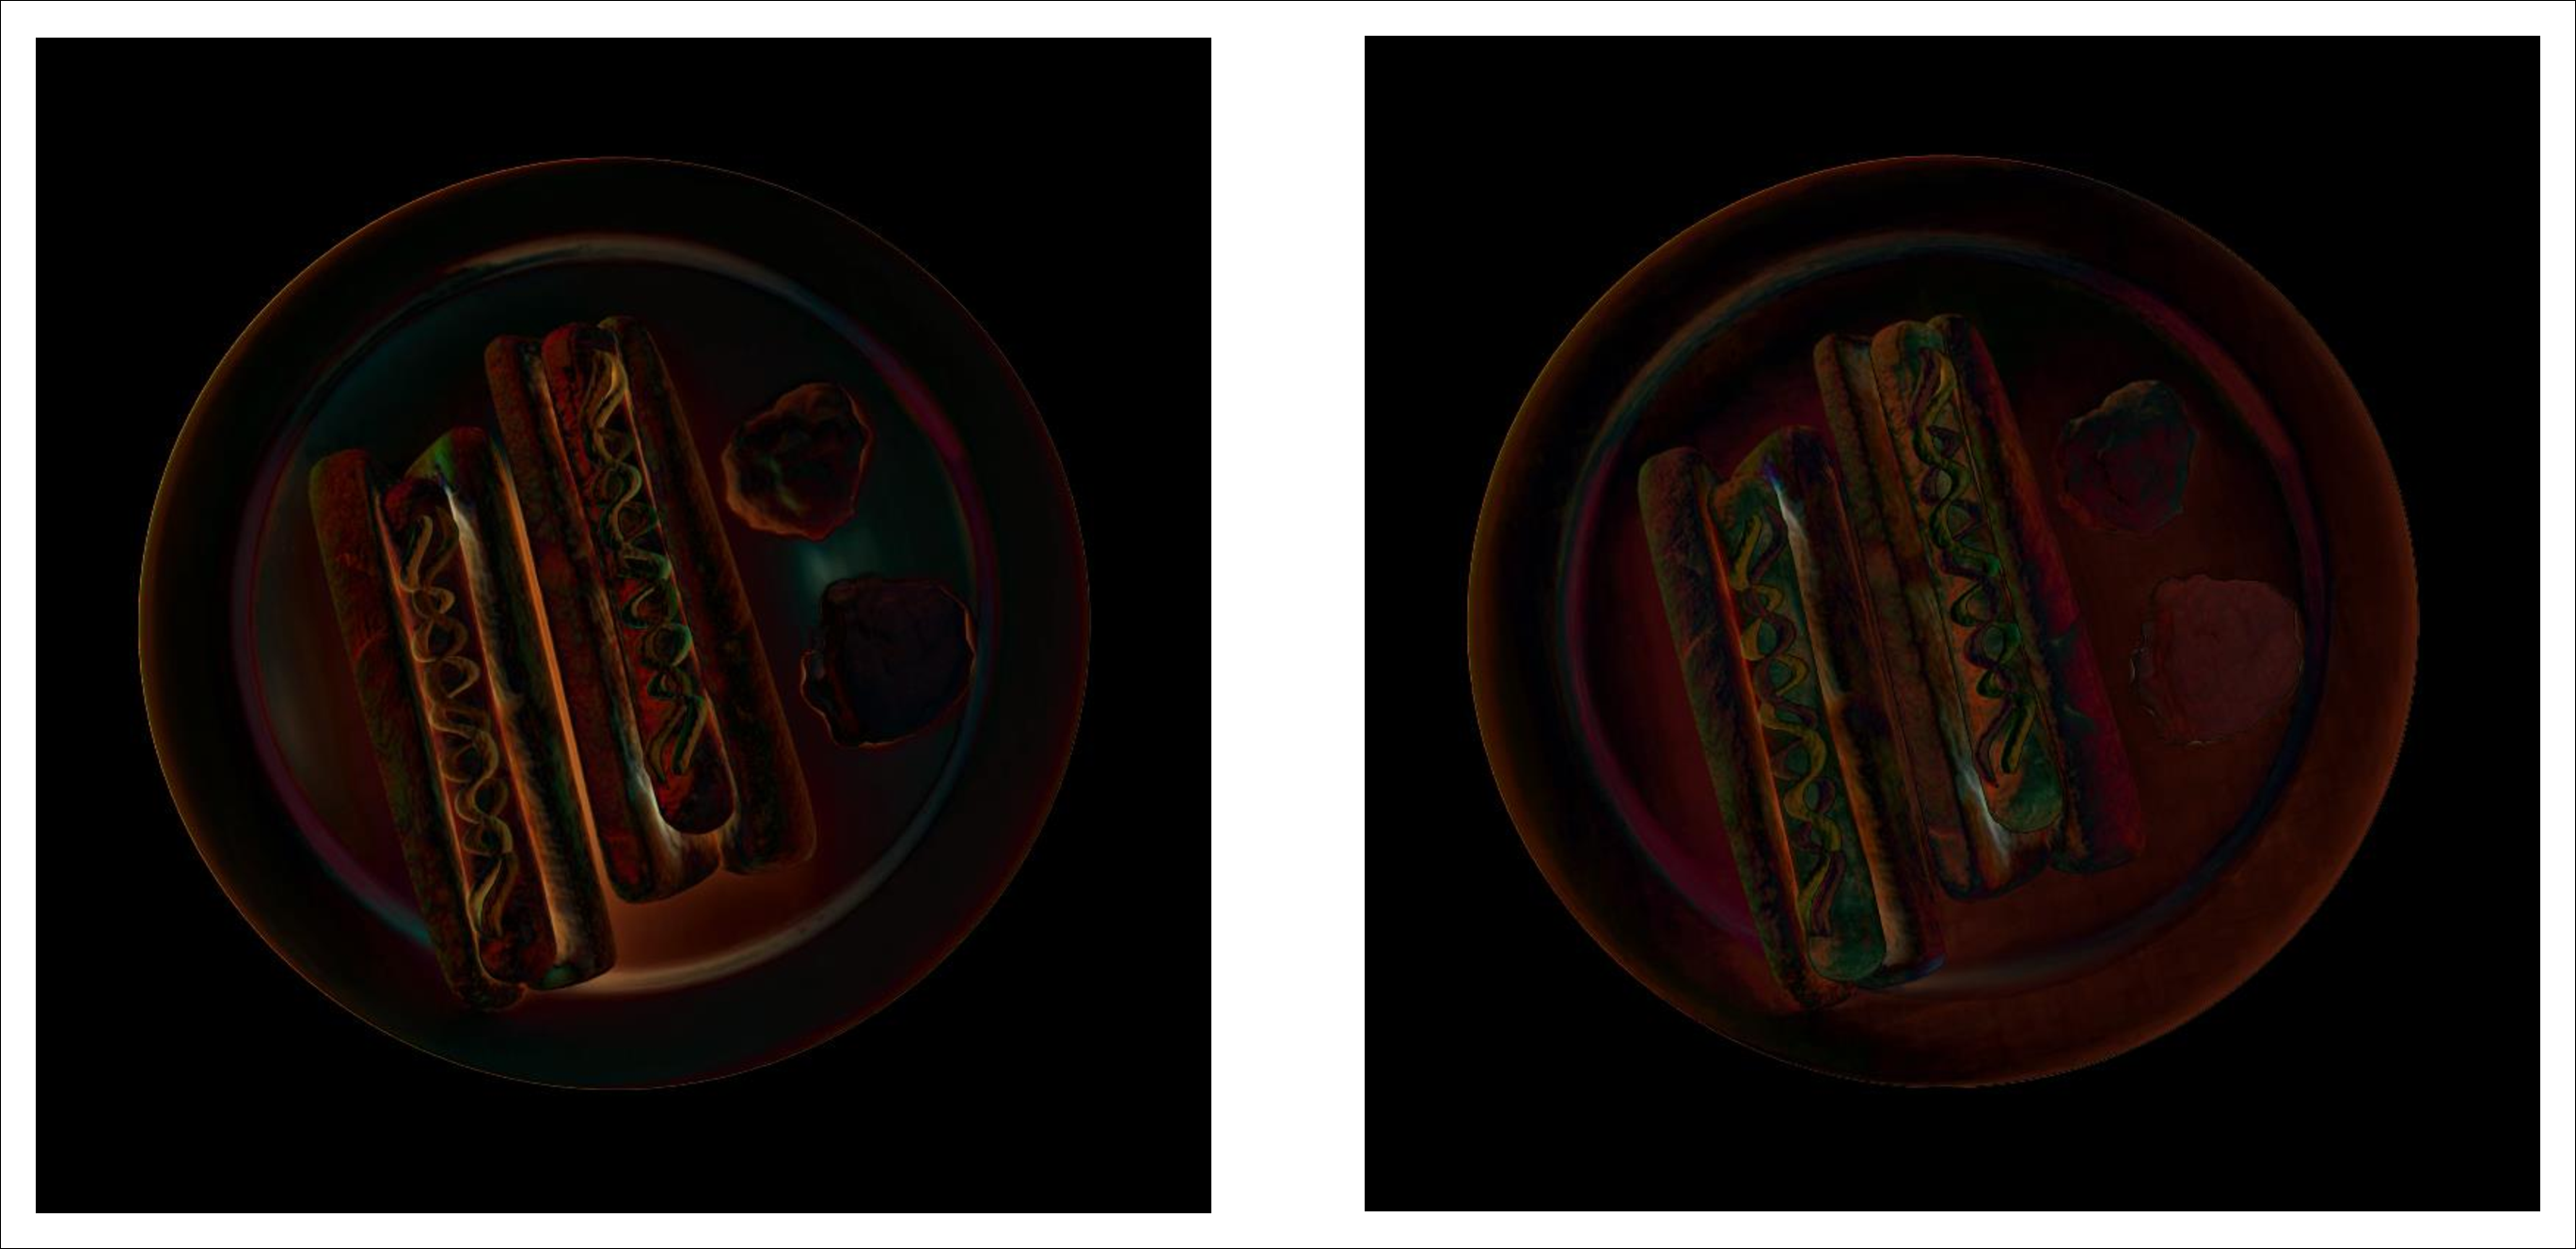
\includegraphics[width=0.81\linewidth]{diff.pdf}
  \caption{漫反射颜色比较2}
  \label{fig:diff}
\end{figure}

这一阶段训练的效果可以在图 \ref{fig:diff} 中更明显地看到。我们将加入第三阶段训练前后的漫反射颜色,在经过颜色修正后,直接与真实漫反射颜色作差得到图中的两张图片。可以看到,左图中有明显的亮区,对应着原图中照明伪影较多的区域。右图中则相对较少。